\section{Procedimento \& Analisi Dati}

Poichè stiamo lavorando in ambito di ottica geometrica e le leggi che andremo ad applicare, quella del costruttore di lenti e la legge dei punti coniugati, dobbiamo fare alcune assunzioni relative all'apparato.
L'ipotesi fondamentale sulla quale si basa tutta l'esperieza e che i raggi luminosi incidenti sulle nostre lenti siano raggi parassiali, ovvero ci dobbiamo porre nell'ipotesi di raggi lontani.
Inoltre per non appesantire la lettura nel seguito indicheremo con queste lettere le seguenti quantità:

%\begin{figure}[b!]
%	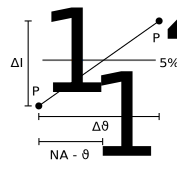
\includegraphics[width=16cm]{drawing.pdf}
%\end{figure}

\begin{equation*}
	p \,=\, \text{distanza tra il cento della lente e la posizione dell'oggetto}
\end{equation*}
\begin{equation*}
	q \,=\, \text{distanza tra il cento della lente e la posizione dell'immagine}
\end{equation*}
\begin{equation*}
	f \,=\, \text{fuoco della lente analizzata}
\end{equation*}
\begin{equation*}
	h \ped{imm} \,=\, \text{altezza dell'immagine sullo schermo}
\end{equation*}
\begin{equation}
	\text{Legge dei puni coniugati:} \qquad \frac{1}{f} \,=\, \frac{1}{p} + \frac{1}{q}
	\label{coniugati}
\end{equation}
\begin{equation}
	\text{Legge del costruttore di lenti:} \qquad \frac{1}{f} \,=\, (n-1)\left(\frac{1}{R\ped{1}}-\frac{1}{R\ped{2}}\right)
	\label{costruttore}
\end{equation}


\subsection{Fuoco della lente convergente}

Come primo obbiettivo ci siamo posti quello di calcolare il fuoco della lente convergente. Per ottenere questo riultato abbiamo misurato per dodici volte il valore che il parametro $q$ assume al variare del parametro $p$. Tenendo ferma la sorgente luminosa, abbiamo incrementato di volta in volta la distanza tra la lente e la sorgente luminosa e di seguito abbiamo rilevato il valore di $q$ mettendo a fuoco l'immagine proiettata sullo schermo.

E' importante sottolineare che nel caso in cui l'immagine si è formata ad una grande distanza dalla lente, riuscire a mettere a fuoco non è stato semplice a causa dell'effetto di profondità di campo. Abbiamo deciso quindi di prendere due misure di $q$. Infatti una volta che l'immagine ci sembrava essere a fuoco abbiamo mosso lo schermo in avanti e in dietro in modo da avere l'immagine leggermente fuori fuoco in entrambe le situazioni e abbiamo preso questi due valori. Facendone la media di questi due valori dovremmo ottenere un valore più probabile per la nostra variabile $q$, rispetto ad un singolo valore preso quando l'immagine è a ``fuoco''.

Una volta ottenuti i valori  di $p$ e $q$, abbiamo calcolato per ognuno il relativo valore di $f$ e infine ne abbiamo fatto una media.
Il valore della focale $f$ della lente convergente ottenuto è:

\begin{equation}
	f \ped{div} \,=\, XXX
\end{equation}

Inoltre vogliamo ricavare il valore della magnificazione per ogni coppia $p$ e $q$. Ricordiamo che la magnificazione è il rapporto tra le dimensioni dell'immagine ottenuta ($h \ped{imm}$) rispetto alle dimensioni reali dell'oggetto ($h$).

\begin{equation}
	m_{1} \,=\, \frac{h \ped{imm}}{h}
\end{equation}

Infine per avere una verifica della correttezza dei dati da noi presi possiamo mettere a confronto il valore della magnificazione trovato empiricamente con quello che si può ricavare dalla seguente relazione:

\begin{equation}
	m_{2} \,=\, \frac{q}{p}
\end{equation}

[Tabella m e m\']

Come si può osservare dai dati in tabella i due valori della magnificazione ricavati con entrambi i procedimenti risultano compatibili entro i propri errori. 

\subsection{Aberrazione cromatica relativa alla lente convergente}

Per valutare e osservare il fenomeno dell'aberrazione cromatica per la lente convergente abbiamo calcolato grazie alla relazione (\ref{coniugati}) il fuoco relativo ai raggi luminosi monocromatici rossi e blu. Per ottenere i raggi monocromatici non abbiamo fatto altro che porre un vetrino colorato difronte alla sorgente luminosa. I valori di $p$ e $q$ sono stati presi seguendo lo stesso procedimento adottato per la lente convergente, salvo il fatto che è stato preso solo un valore dei due parametri.
I risultati da noi ottenuti sono riportati nella tabella sottostante:

[TABELLA!!!]

Come si può notare dai dati in tabella i valori per il fuoco della lente convergente sono differerenti a seconda della lunghezza d'onda (colore) dei raggi luminosi incidenti su quest'ultima. 









